\section{Priprava okolja}\label{sec:1}
Podatki so shranjeni v formatu \verb|.root|. To je format, ki ga je razvil CERN
za shranjevanje in analizo velikih količin podatkov v fiziki delcev. Te datoteke
so zelo učinkovite pri obdelavi in shranjevanju kompleksnih podatkovnih struktur,
kot so histogrami, drevesa in grafi.
Za odpiranje datotek \verb|.root| potrebuješ programsko opremo \verb|ROOT|, ki je
javno dostopna na portalu CERN-a.
\\
\\
Izkaže se, da za enostavno branje datotek v \verb|pythonu|, ne potrebuješ celotnega modula, ampak
le pomožno knjižico \verb|uproot|, ki je veliko manjša od celotnega \verb|ROOT|-a, kar ne
pomeni, da ni bil uporaben v mojem primeru. Namreč dani podatki so imeli izredno slabo
dokumentacijo in ker sem se sam prvič srečal s takim formatom in knjižicami, mi je prav prišel ukaz
\verb|TBrowser|
v okolju \verb|root|, ker je skoraj razčistil pomen podatkov.
\\
\begin{figure}[h]
    \begin{center}
        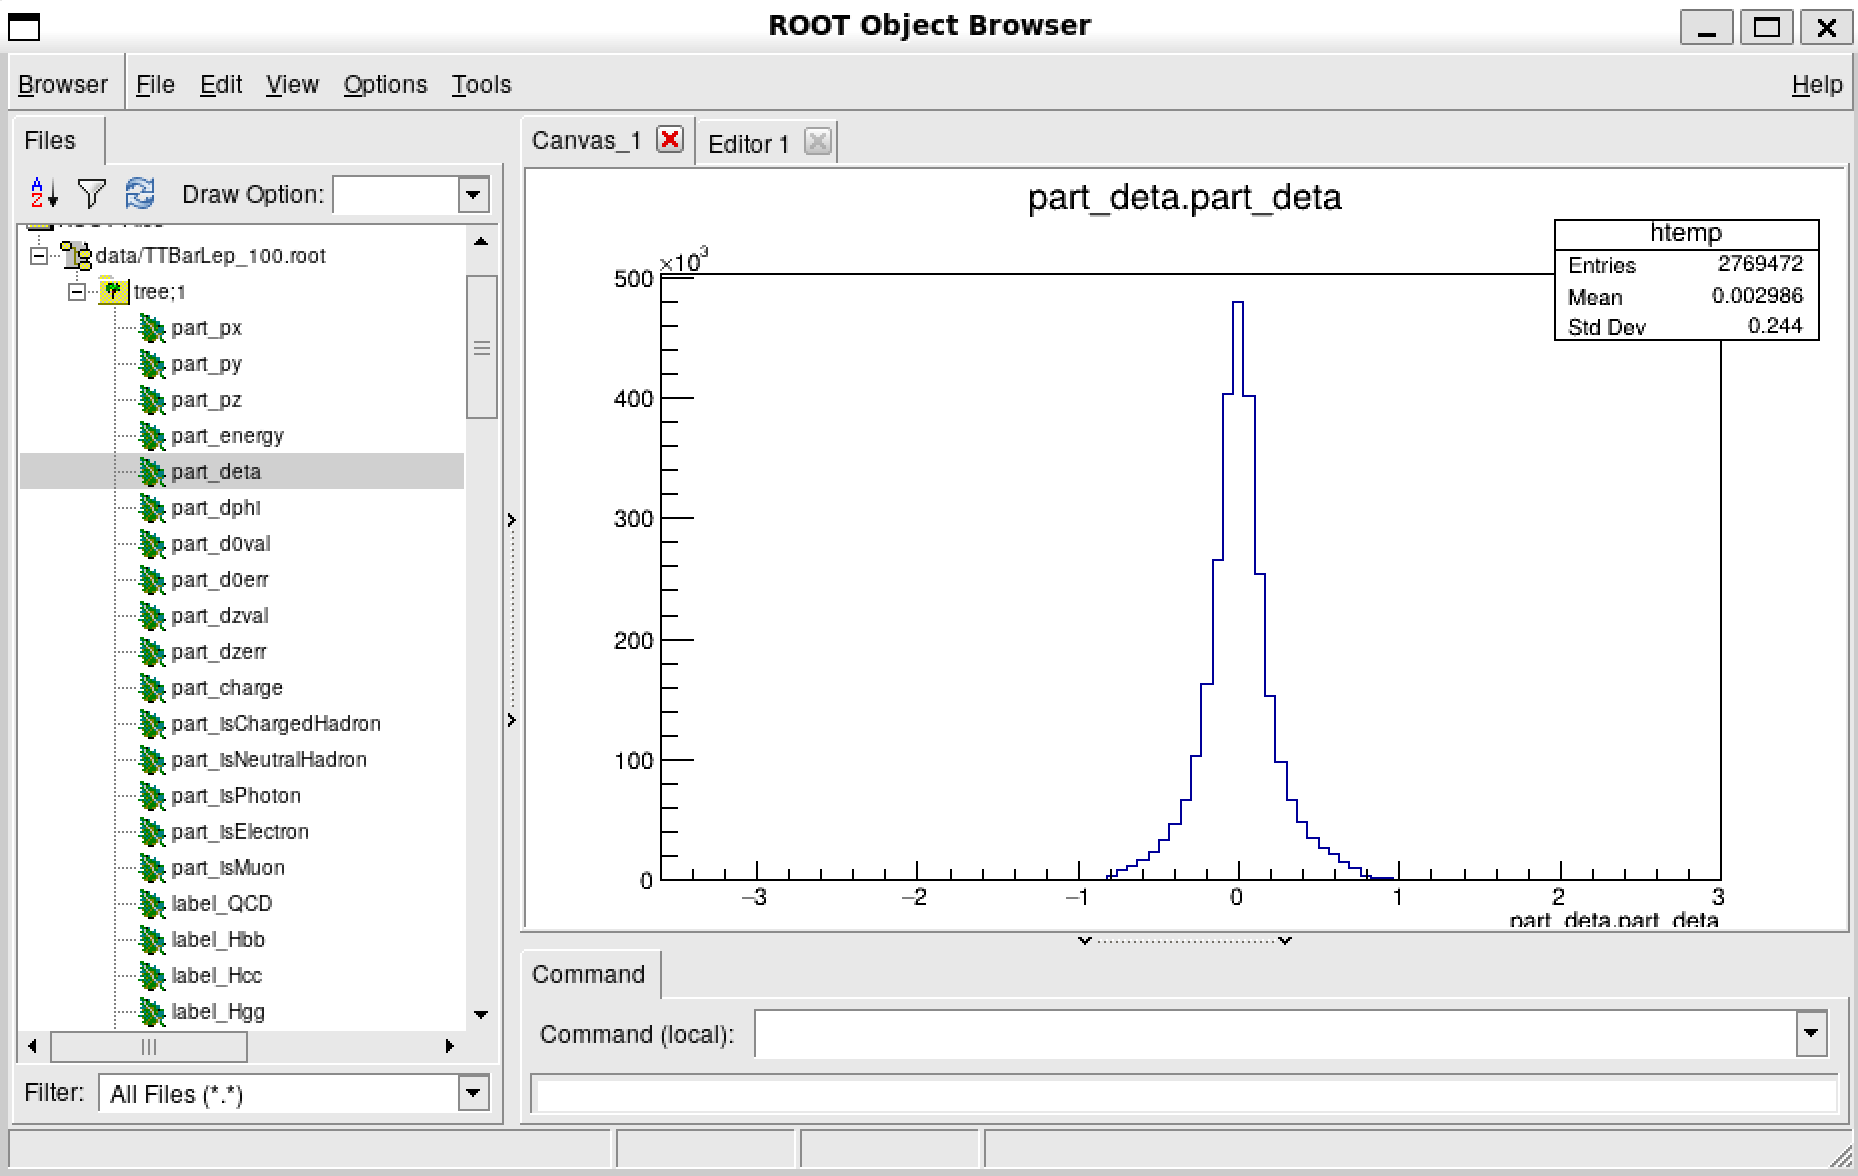
\includegraphics[width=13cm]{sections/section1/figures/TBrowser.png}
        \caption{Grafični prikaz datoteke TTBarLep\_100.root}
        \label{slika 1}
    \end{center}
\end{figure}
\\
\\
Grafična upodobitev zavaja, saj drevo \verb|tree;1| ima veje, ki
jih interpretira kot liste. To se vidi s pomočjo \verb|ipython|-a in
knjižico \verb|uproot|, a to ni tako ključnega pomena.
\\
\\
\newpage \noindent
Zagon programov je odvisen od nekaterih knjižnic. Priporočam, da se knjižnice
inštalira v virtualnem okolju \verb|venv|, ki ga ustvarimo z ukazom \verb|python3 -m venv ./venv|.
Vstop v okolje pa je odvisen od sistema uporabnika, recimo za \verb|linux| lahko uporabimo
ukaz \verb|source ./venv/bin/activate|. Sedaj lahko inštaliramo potrebne knjižnice
za delovanje programov \verb|pip install numpy matplotlib uproot tqdm scipy|. Za nekaterih knjižnic
\verb|pip| ne bo znal sam namestiti, zato jih bo potrebno ročno.
\\
\\
Za branje podatkov sem uporabljal tole kodo.
% #v vsakem jet-u so delci in njihove gibalne količine
\begin{figure}[h]
\begin{lstlisting}[language=Python]
tree = uproot.open(file)['tree']
jets = {}
components = ['px', 'py', 'pz']

for component in components:
    part = 'part_'+component
    branch = tree[part]
    jets[component] = [jet for jet in branch.array().tolist()]

\end{lstlisting}
\end{figure}
Koda je precej počasna, zaradi osme vrstice, ker prevaja podatke iz \verb|.root|
reprezentacije v \verb|numpy| in nato še v navaden seznam. Za pohitritev bi morali
uporabljati jezik C++ in knjižnico \verb|ROOT|, ki ne potrebuje prevajanja v treh korakih ampak samo v enem.
Kompleksnost in berljivost programske kode se veliko bolj poslabša. 

% Sam sem uporabljal \verb|WSL (Windows subsystem for linux)|
% in virtualno okolje \verb|conda|, s katerim sem se izognil packanju celotnega sistema.
